\providecommand{\setflag}{\newif \ifwhole \wholefalse}
\setflag
\ifwhole\else

% Typography and geometry ----------------------------------------------------
\documentclass[letterpaper]{scrbook}
\usepackage[inner=3cm,top=2.5cm,outer=3.5cm]{geometry}

\renewcommand\familydefault{bch}
\usepackage[utf8]{inputenc}
\usepackage{microtype}
\usepackage[small]{caption}
\usepackage[small]{titlesec}
\raggedbottom

% Graphics -------------------------------------------------------------------
\usepackage[pdftex]{graphicx}
\graphicspath{{_include/}}
\DeclareGraphicsExtensions{.png,.pdf}

% Code formatting ------------------------------------------------------------
\usepackage{fancyvrb}
\usepackage{courier}
\usepackage{listings}
\usepackage{color}
\usepackage{alltt}


\definecolor{comment}{rgb}{0.60, 0.60, 0.53}
\definecolor{background}{rgb}{0.97, 0.97, 1.00}
\definecolor{string}{rgb}{0.863, 0.066, 0.266}
\definecolor{number}{rgb}{0.0, 0.6, 0.6}
\definecolor{variable}{rgb}{0.00, 0.52, 0.70}
\lstset{
  basicstyle=\ttfamily,
  keywordstyle=\bfseries, 
  identifierstyle=,  
  commentstyle=\color{comment} \emph,
  stringstyle=\color{string},
  showstringspaces=false,
  columns = fullflexible,
  backgroundcolor=\color{background},
  mathescape = true,
  escapeinside=&&,
  fancyvrb
}
\newcommand{\code}[1]{\lstinline!#1!}
\newcommand{\f}[1]{\lstinline!#1()!}



% Links ----------------------------------------------------------------------

\usepackage{hyperref}
\definecolor{slateblue}{rgb}{0.07,0.07,0.488}
\hypersetup{colorlinks=true,linkcolor=slateblue,anchorcolor=slateblue,citecolor=slateblue,filecolor=slateblue,urlcolor=slateblue,bookmarksnumbered=true,pdfview=FitB}
\usepackage{url}

% Tables ---------------------------------------------------------------------
\usepackage{longtable}
\usepackage{booktabs}

% Miscellaneous --------------------------------------------------------------
\usepackage{pdfsync}
\usepackage{appendix}

\usepackage[round,sort&compress,sectionbib]{natbib}
\bibliographystyle{plainnat}


\title{ggplot2}
\author{Hadley Wickham}

\begin{document}
\fi


% SET_DEFAULTS
%   GG-WIDTH: 4  GG-HEIGHT: 4
%   TEX-WIDTH: 0.5\textwidth
%   INLINE: FALSE
%   CACHE: TRUE
% 

% END

\chapter{Mastering the grammar}
\label{cha:mastery}

\section{Introduction}

You can choose to use just \f{qplot}, without any understanding of the underlying grammar, but you will not be able to use the full power of ggplot.  By learning more about the grammar, and the components that make it up, you will be able to create a wider range of plots, as well as being able to combine multiple sources of data, and customise to your heart's content.  You may want to skip this chapter in a first reading of the book, coming back to it when you want a deeper understanding of how all the pieces fit together.

This chapter describes the theoretical basis of \ggplot: the layered grammar of graphics.  The layered grammar is based on Wilkinson's grammar of graphics \citep{wilkinson:2006}, but adds a number of enhancements that help it to be more expressive and fit smoothly into the R environment.  The differences between the layered grammar and Wilkinson's grammar are described fully in \citep{wickham:2008}, and a guide for converting between {\sc gpl} and \ggplot is included in Appendix~\ref{chp:translating}.  In this chapter you will learn a little bit about each component of the grammar and how they all fit together.  The next chapters discuss the components in more detail, and provide more examples of how you can use them in practice.

This chapter begins by describing in detail the process of drawing a simple plot.  Section~\ref{sec:simple-plot} start with a simple scatterplot, then in Section~\ref{sec:complex-plot} make it more complex by adding a smooth line and facetting.  While working through these examples you will be introduced to all six components of the grammar, which are then defined more precisely in Section~\ref{sec:components}.  The chapter concludes with Section~\ref{sec:data-structures}, which describes how the various components map to data structures in R.  

\section{Fuel economy data}
\label{sec:fuel_economy_data}

Consider the fuel economy dataset illustrated in Table~\ref{tbl:mpg}.  It records make, model, class, engine size, transmission and fuel economy for a selection of US cars in 1999 and 2008.  It contains the 38 models that had a new release every year, an indicator that the car was a popular model.  These models are the Audi A4, Audi A4 Quattro, Audi A6 Quattro, Chevrolet C1500 Suburban 2wd, Chevrolet Corvette, Chevrolet K1500 Tahoe 4wd, Chevrolet Malibu, Dodge Caravan 2wd, Dodge Dakota Pickup 4wd, Dodge Durango 4wd, Dodge Ram 1500 Pickup 4wd, Ford Expedition 2wd, Ford Explorer 4wd, Ford F150 Pickup 4wd, Ford Mustang, Honda Civic, Hyundai Sonata, Hyundai Tiburon, Jeep Grand Cherokee 4wd, Land Rover Range Rover, Lincoln Navigator 2wd, Mercury Mountaineer 4wd, Nissan Altima, Nissan Maxima, Nissan Pathfinder 4wd, Pontiac Grand Prix, Subaru Forester Awd, Subaru Impreza Awd, Toyota 4runner 4wd, Toyota Camry, Toyota Camry Solara, Toyota Corolla, Toyota Land Cruiser Wagon 4wd, Toyota Toyota Tacoma 4wd, Volkswagen Gti, Volkswagen Jetta, Volkswagen New Beetle, and Volkswagen Passat.  This data was collected from the EPA fuel economy website, \url{http://fueleconomy.gov}.

% source("latex.r")
% cat(tabulate(mpg[1:10, -6]))
\begin{table}
  \begin{center}
  \begin{tabular}{llrrrlrrl}
    \toprule
    manufacturer & model & disp & year & cyl & cty & hwy & class \\
    % Model & Manufacturer & Displacement (l) & Year & Cylinders & City mpg & Highway mpg & Class \\
    \midrule
    audi & a4         & 1.8 & 1999 & 4 & 18 & 29 & compact\\
    audi & a4         & 1.8 & 1999 & 4 & 21 & 29 & compact\\
    audi & a4         & 2.0 & 2008 & 4 & 20 & 31 & compact\\
    audi & a4         & 2.0 & 2008 & 4 & 21 & 30 & compact\\
    audi & a4         & 2.8 & 1999 & 6 & 16 & 26 & compact\\
    audi & a4         & 2.8 & 1999 & 6 & 18 & 26 & compact\\
    audi & a4         & 3.1 & 2008 & 6 & 18 & 27 & compact\\
    audi & a4 quattro & 1.8 & 1999 & 4 & 18 & 26 & compact\\
    audi & a4 quattro & 1.8 & 1999 & 4 & 16 & 25 & compact\\
    audi & a4 quattro & 2.0 & 2008 & 4 & 20 & 28 & compact\\
        \bottomrule
  \end{tabular}
  \end{center}
  \caption{The first 10 cars in the \code{mpg} data set, included in the \ggplot package.  \var{cty} and \var{hwy} record miles per gallon (mpg) for city and highway driving respectively.  }
  \label{tbl:mpg}
\end{table}

This dataset suggests many interesting questions.  How are engine size and fuel economy related?  Has fuel economy improved in the last ten years?  We will try to answer the first question and in the process learn more detail about how the scatterplot is created.

\section{Building a scatterplot}
\label{sec:simple-plot}

Consider Figure~\ref{fig:mpg}, one attempt to answer this question.  It is a scatterplot of two continuous variables, with points coloured by a third variable.  From your experience in the previous chapter, you should have a pretty good feel for how to create this plot with \f{qplot}.  But what is going on underneath the surface?  How does \ggplot draw this plot?

% FIGURE
%   LABEL: mpg
%   GG-WIDTH: 8 GG-HEIGHT: 4 TEX-WIDTH: \textwidth
%   CAPTION: A scatterplot of engine displacement in litres (displ) vs
%   average highway miles per gallon (hwy).  Points are coloured according
%   to number of cylinders.  This plot summarises the most important
%   factor governing fuel economy: engine size
% 
% qplot(displ, hwy, data=mpg, colour=factor(cyl))
% 
\input{_include/4c60951bf8e60507a206c983469d3dc6.tex}
% END

\subsubsection{Mapping aesthetics to data}

What is a scatterplot?  You have seen many before and have probably even drawn some by hand.  A scatterplot represents each observation as a point (•), positioned according the value of two variables.  As well as a horizontal and vertical position, each point also has a size, a colour and a shape. These attributes are called called {\bf aesthetics}, and are the properties that can perceived on the graphic.  Each aesthetic can be mapped to a variable, or set to a constant value.  In Figure~\ref{fig:mpg} $x$-position is mapped to \var{displ}, $y$-position to \var{hwy} and colour to \var{cyl}.  Size and shape are not mapped to variables, but remain at their (constant) default values.  

Once we have these mappings we can create a new dataset that records this information.  Table~\ref{tbl:mapping} shows the first 10 rows of the data behind Figure~\ref{fig:mpg}.  This new dataset encapsulates the combination of the original data and the aesthetic mappings.  We can create many different types of plots using this data.  The scatterplot uses points, but we were instead to draw lines we would get a line plot.  If we used bars, we'd get a bar plot.  Neither of those examples make sense for this data, but we could still draw them, as in Figure~\ref{fig:other-geoms}.  Much like in English, using \ggplot it is still possible to produce grammatically valid plots that don't make any sense.

% scatter <- with(mpg, data.frame(x = displ, y = hwy, colour = cyl))
% cat(tabulate(scatter[1:10, ]))
\begin{table}[ht]
  \begin{center}
  \begin{tabular}{rrr}
    \toprule
    \code{x} & \code{y} & \code{colour}\\
    \midrule
    1.8 & 29 & 4\\
    1.8 & 29 & 4\\
    2.0 & 31 & 4\\
    2.0 & 30 & 4\\
    2.8 & 26 & 6\\
    2.8 & 26 & 6\\
    3.1 & 27 & 6\\
    1.8 & 26 & 4\\
    1.8 & 25 & 4\\
    2.0 & 28 & 4\\
    \bottomrule
  \end{tabular}
  \end{center}
  \caption{First 10 rows from \code{mpg} rearranged into format for scatterplot.  This is all the information we need to draw the scatterplot.}
  \label{tbl:mapping}
\end{table}

% FIGURE
%   LABEL: other-geoms
%   CAPTION: Instead of using points to represent the data, we could use
%   other geoms like, \leftc lines or, \rightc bars.  Neither of these geoms
%   make much sense for this data, but they are still valid graphics.
% 
% qplot(displ, hwy, data=mpg, colour=factor(cyl), geom="line") + 
%   opts(drop = "legend_box")
% qplot(displ, hwy, data=mpg, colour=factor(cyl), geom="bar", 
%   stat="identity", position = "identity") + 
%   opts(drop = "legend_box")
\input{_include/f71ee365a5fd9c8ef5db9bf636da4748.tex}
% END

Bars, lines and points are all examples of geometric objects, or {\bf geom}s. Geoms determine the ``type'' of the plot. Plots that use a single geom are often given a special name, a few of which are listed in Table~\ref{tbl:named-plots}. More complex plots with combinations of multiple geoms don't have a special name, and we have to describe them by hand. For example, Figure~\ref{fig:complex-plot} overlays a per group regression line on the existing plot. What would you call this plot?   Once you've mastered the grammar, I think you'll find that most of the plots that you produce are uniquely tailored to your problems and will no longer have common names.

\begin{table}
  \begin{center}
  \begin{tabular}{lll}
    \toprule 
    Named plot & Geom & Other features \\
    \midrule
    scatterplot & point &  \\
    bubblechart & point & size mapped to a variable \\ 
    barchart & bar &  \\
    box and whiskers plot & boxplot &  \\
    line chart & line &  \\     
    \bottomrule
  \end{tabular}
  \end{center}
  \caption{A selection of named plots and the geoms that they correspond to.}
  \label{tbl:named-plots}
\end{table}

% FIGURE
%   LABEL: complex-plot
%   GG-WIDTH: 8 GG-HEIGHT: 4 TEX-WIDTH: \textwidth
%   CAPTION: More complicated plots don't have their own names.  This plot
%   takes Figure~\ref{fig:mpg} and adds a regression line to each group. 
%   What would you call this plot?
% 
% qplot(displ, hwy, data=mpg, colour=factor(cyl)) + 
% geom_smooth(data= subset(mpg, cyl != 5), method="lm")
\input{_include/dada1840f3571fba4c004c9ffea92609.tex}
% END

\subsubsection{Scaling} 

The values in Table~\ref{tbl:mapping} have no meaning to the computer.  We need to convert them from data units (e.g.\ litres, miles per gallon and number of cylinders) to physical units (e.g.\ pixels and colours) that the computer can display.  This conversion process is called {\bf scaling} and performed by (surprise!) scales.   Appendix~\ref{chp:specification} describes the way that specifies values for colours, sizes, shapes and so on.

For scales that control the horizontal and vertical position, we need an additional step which determines how the two positions (x and y) combine to form the final position on the plot.  This is done by the coordinate system, or {\bf coord}.  In most cases this will be Cartesian coordinates, but it might by polar coordinates, or a spherical projection used for a map.

Scaling position is easy in this example because we are using the default  linear scales and Cartesian coordinate system.  We only need a linear mapping from the range of the data to $[0, 1]$.  We use $[0, 1]$ instead of exact pixels because the drawing system that \ggplot uses, \code{grid}, takes care of that final conversion. 

The process for mapping the colour is a little more complicated, as we have a  non-numeric result: colours.  However, colours can be parameterised numerically, typically with three values.  For discrete values, the default colour scale maps the  to evenly spaced hues on a colour wheel, as shown in  Figure~\ref{fig:colour-wheel}.

\begin{figure}[htbp]
  \centering
    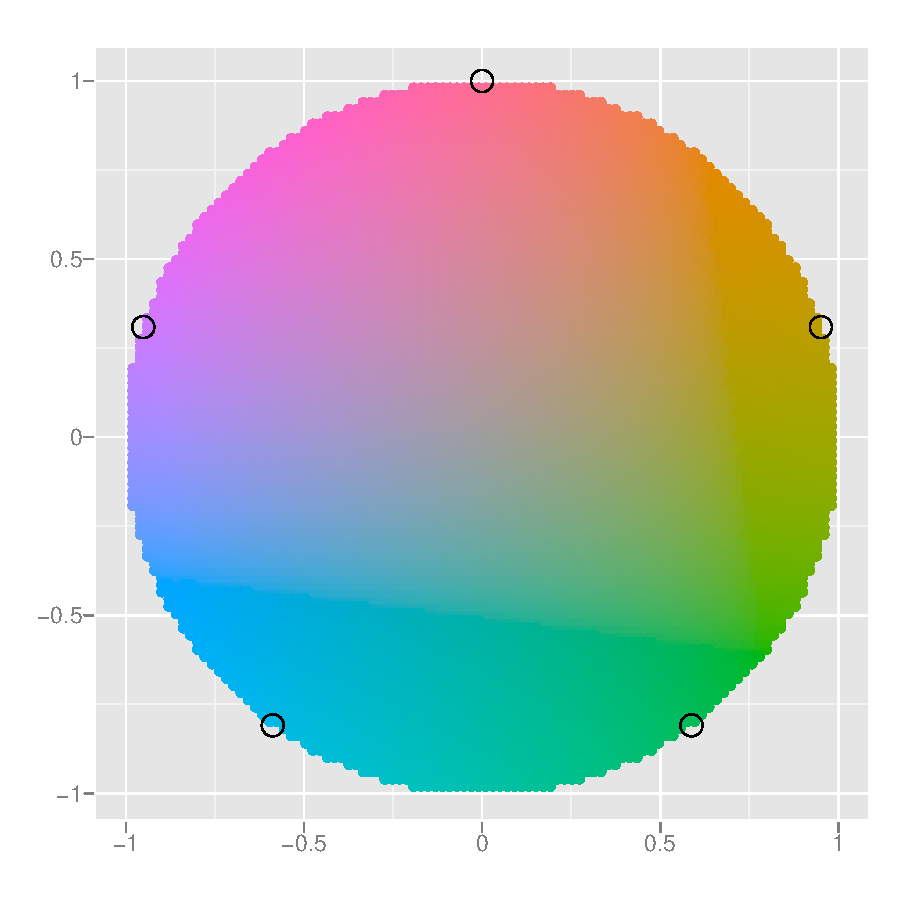
\includegraphics[width=3in]{colour-wheel.pdf}
  \caption{A colour wheel showing how the default colour scheme for discrete values is produced.}
  \label{fig:colour-wheel}
\end{figure}

The result of these conversions is Table~\ref{tbl:scaled}, which contains values that have meaning to the computer.  As well as the variables from the aesthetic mapping, we have also included the default values for the geom.  We need these so that the aesthetics for each point are completely specified.

% Colour the entries by their actual colour

% scaled <- transform(scatter,
%   x = format(rescaler(x, "range"), digits=2),
%   y = format(rescaler(y, "range"), digits=2)
% )
% col <- scale_colour_discrete()
% col$train(factor(scaled$colour))
% scaled$colour <- col$map(factor(scaled$colour))
% scaled$size <- 1
% scaled$shape <- 20
% cat(tabulate(scaled[1:10, ]))

\definecolor{ff6c91}{rgb}{1.00, 0.42, 0.57}
\definecolor{00c1a9}{rgb}{0.00, 0.76, 0.66}

\begin{table}[ht]
  \begin{center}
  \begin{tabular}{rrrrr}
    \toprule
    \code{x} & \code{y} & \code{colour} & \code{size} & \code{shape}\\
    \midrule
    0.037 & 0.531 & {\color{ff6c91} \#FF6C91} & 1 & 20 \\
    0.037 & 0.531 & {\color{ff6c91} \#FF6C91} & 1 & 20 \\
    0.074 & 0.594 & {\color{ff6c91} \#FF6C91} & 1 & 20 \\
    0.074 & 0.562 & {\color{ff6c91} \#FF6C91} & 1 & 20 \\
    0.222 & 0.438 & {\color{00c1a9} \#00C1A9} & 1 & 20 \\
    0.222 & 0.438 & {\color{00c1a9} \#00C1A9} & 1 & 20 \\
    0.278 & 0.469 & {\color{00c1a9} \#00C1A9} & 1 & 20 \\
    0.037 & 0.438 & {\color{ff6c91} \#FF6C91} & 1 & 20 \\
    0.037 & 0.406 & {\color{ff6c91} \#FF6C91} & 1 & 20 \\
    0.074 & 0.500 & {\color{ff6c91} \#FF6C91} & 1 & 20 \\
    \bottomrule
  \end{tabular}
  \end{center}
  \caption{Simple dataset with variables mapped into aesthetic space.  Default values for other aesthetics are also included: the points will be filled circles (shape 20 in R) with a 1mm diameter.}
  \label{tbl:scaled}
\end{table}

Finally, we need to render this data to create the graphical objects that are displayed on the screen.  To create a complete plot we need to combine graphical objects from three sources:  \emph{data}, represented by the point geom; \emph{scales and coordinate system}, which generate axes and legends so that we can read values from the graph; and \emph{plot annotations}, such as the background and plot title.  Figure~\ref{fig:empty} removes the contribution of the data to show what elements the scales and plot contribute.

\begin{figure}[htbp]
  \centering
  \caption{Contributions from the scales, the axes and legend and grid lines, and the plot background.  Contributions from the data, the point geom, has been removed.}
  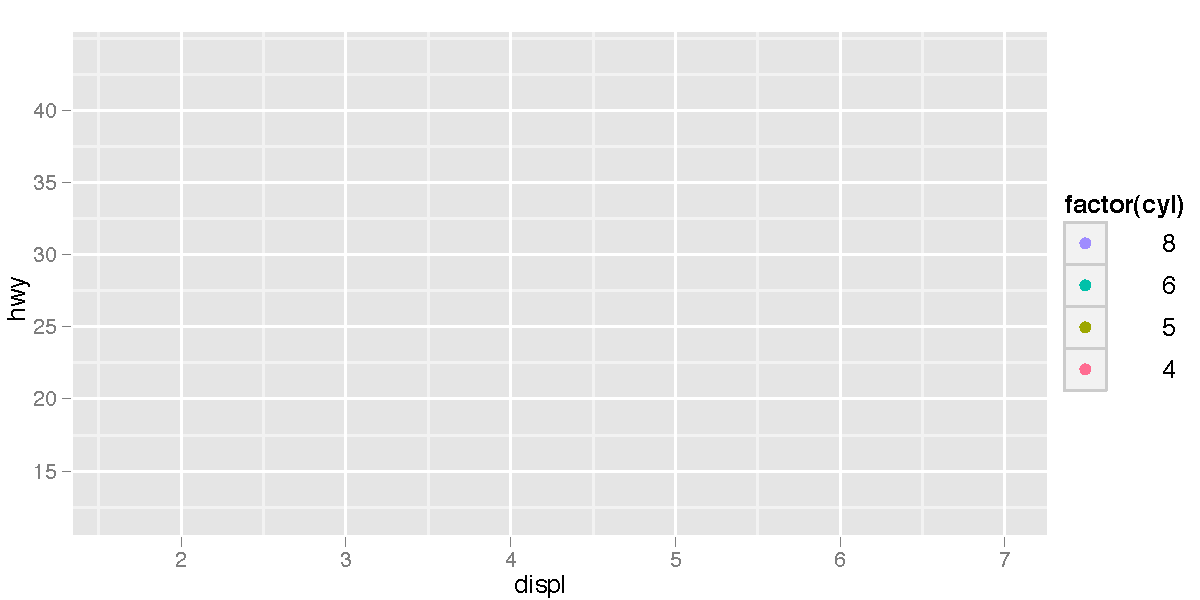
\includegraphics[width= \textwidth]{empty}
  \label{fig:empty}
\end{figure}

\section{A more complicated plot}
\label{sec:complex-plot} 

With a simple example under our belts, it's now turn to look at the slightly more complicated plot in Figure~\ref{fig:complex}.  This plot adds three new components to the mix: facets, multiple layers and statistics.  The facets and layers expand the data structure a little:  each panel in each layer has its own dataset.  Think of this like a 3d array of data frames.  The smooth stat adds an addition step in the above process: after mapping the data to aesthetics, the relationship between the x and y variables is summarised with a flexible model.  Other use statistical transformations include binning, for the histogram, and ...

% FIGURE
%   GG-WIDTH: 8 GG-HEIGHT: 4 TEX-WIDTH: \textwidth
%   LABEL: complex
%   CAPTION: A more complex plot with facets and multiple layers.
% 
% qplot(displ, hwy, data=mpg, facets = . ~ year) + geom_smooth()
\input{_include/c2c66c5100435463277a6e99dd4af40a.tex}
% END

Facetting splits the original dataset into a dataset for each subset, so the data that underlies Figure~\ref{fig:complex} looks like Table \ref{tbl:complex}.

\begin{table}[ht]
  \centering
  \begin{tabular}{r|r|r|r}
    & $x$ & $y$ & $colour$\\
    \hline
    a & 2 & 4 & red\\
    a & 1 & 1 & red\\
    \hline \hline
    b & 4 & 15 & blue\\
    b & 9 & 80 & blue
  \end{tabular}

  \caption{Simple dataset faceted into subsets.}
  \label{tbl:complex}
\end{table}

The first steps of plot creation proceed as before, but new steps are necessary when we get to the scales.   Scaling actually occurs in three parts: transforming, training and mapping. 

\begin{itemize}
  \item  Scale transformation occurs before statistical transformation so that statistics are computed on the scale-transformed data.  This ensures that a plot of $log(x)$ vs $log(y)$ on linear scales looks the same as $x$ vs $y$ on log scales.  See Section~\ref{sub:transformation} for more details. Transformation is only necessary for non-linear scales, because all statistics are location-scale invariant.

  \item After the statistics are computed, each scale is trained on every faceted dataset (a plot can contain multiple datasets, e.g.\ raw data and predictions from a model).  The training operation combines the ranges of the individual datasets to get the range of the complete data.  If scales were applied locally, comparisons would only be meaningful within a facet.  This is shown in Table \ref{tbl:complex-incorrect}.

  % FIXME
  \item Finally the scales map the data values into aesthetic values.  This gives Table \ref{tbl:complex-mapping} which is essentially identical to Table \ref{tbl:mapping} apart from the structure of the datasets.  Given that we end up with an essentially identical structure you might wonder why we don't simply split up the final result.  There are several reasons for this.  It makes writing statistical transformation functions easier, as they only need to operate on a single facet of data, and some need to operate on a single subset, for example, calculating a percentage.  Also, in practice we may have a more complicated training scheme for the position scales so that different columns or rows can have different $x$ and $y$ scales.  
  
\end{itemize}



\section{Components of the layered grammar}
\label{sec:components}

In the examples above, we have seen some of the components that make up a plot:

\begin{itemize}
  \item data and aesthetic mappings,
  \item geometric objects, 
  \item statistical transformations,
  \item scales,
  \item and facet specification.
\end{itemize}

\noindent And have also touched on the coordinate system.  Together, the data, mappings, statistical transformation and geometric object form a {\bf layer}.  A plot may have multiple layers, as in the example, where we overlaid a  smoothed line on scatterplot.  To be precise, the layered grammar defines the components of a plot as:

\begin{itemize}
  \item A default dataset and set of mappings from variables to aesthetics.
  \item One or more layers, each composed of a geometric object, a statistical transformation, and a position adjustment, and optionally, a dataset and aesthetic mappings.
  \item One scale for each aesthetic mapping used.
  \item A coordinate system.
  \item The facet specification.
\end{itemize}


The layer component is particularly important as it determines the physical representation of the data, with the combination of stat and geom defining many familiar named graphics: the scatterplot, histogram, contourplot, and so.  In practice, many plots have (at least) three layers: the data, context for the data, and a statistical summary of the data.  For example, to visualise a  spatial point process, we might display the points themselves, a map giving some context to the locations of points, and contours of a 2d density estimate.

This grammar is useful for both the user and the developer of statistical graphics.  For the user, it makes it easier to iteratively update a plot, changing a single feature at a time.  The grammar is also useful because it suggests the high level aspects of a plot that \emph{can} be changed, giving us a framework to think about graphics, and hopefully shortening the distance from mind to paper.  It also encourages the use of graphics customised to a particular problem, rather than relying on generic named graphics.

For the developer, it makes it much easier to add new capabilities. You only need to add the one component that you need, and continue to use the all the other existing components.  For example, you can add a new statistical transformation, and continue to use the existing scales and geoms.  It is also useful for discovering new types of graphics, as the grammar effectively defines the parameter space of statistical graphics.

\subsection{Layers}

Layers are responsible for creating the objects that we perceive on the plot.  A layer is composed of four parts:  

\begin{itemize}
  \item data and aesthetic mapping,
  \item a statistical transformation (stat), 
  \item a geometric object (geom)
  \item and a position adjustment.
\end{itemize}

\noindent These parts are described in detail below.

Usually all the layers on a plot have something in common, which is typically that they are different views of the same data, e.g.\ a scatterplot with overlaid smoother.  


\subsubsection{Data and mapping}\label{sub:data_and_mapping} 

Data is obviously a critical part of the plot, but it is important to remember that it is independent from the other components: we can construct a graphic that can be applied to multiple datasets. Data is what turns an abstract graphic into a concrete graphic.

Along with the data, we need a specification of which variables are mapped to which aesthetics.  For example, we might map weight to x position, height to y position and age to size.  The details of the mapping are described by the scales, Section~\ref{sec:scales}.  Choosing a good mapping is crucial for generating a useful graphic, as described in Section~\ref{sec:strategy}.

\subsubsection{Statistical transformation}\label{sub:stats} 

A statistical transformation, or {\bf stat}, transforms the data, typically by summarising it in some manner.  For example, a useful stat is the smoother, which calculates the mean of y, conditional on x, subject to some restriction that ensures smoothness. Table \ref{tbl:statistics} lists some of the stats available in ggplot2.  To make sense in a graphic context a stat must be location-scale invariant: $\mbox{f}(x + a) = \mbox{f}(x) + a$ and $\mbox{f}(b \cdot x) = b \cdot \mbox{f}(x)$.  This ensures that the transformation is invariant under translation and scaling, which are common operations on a graphic.

A stat takes a dataset as input and returns a dataset as output, and so a stat can add new variables to the original dataset.  It is possible to map aesthetics to these new variables.  For example, one way to describe a histogram is as a binning of a continuous variable, plotted with bars whose height is proportional to the number of points in each bin, as described in Section \ref{sub:distribution}.  Another useful example is mapping the size of the lines in a contour plot to the height of the contour.

The actual statistical method used by a stat is conditional on the coordinate system.  For example, a smoother in polar coordinates should use circular regression, and in 3d should return a 2d surface rather than a 1d curve.  However, many statistical operations have not been derived for non-Cartesian coordinates and we so we generally fall back to Cartesian coordinates for calculation, which, while not strictly correct, will normally be a fairly close approximation.  

\begin{table}
  \begin{center}
  \begin{tabular}{l|l}
  Name & Description \\
  \hline
  bin & Divide continuous range into bins, and count number of points in each\\ 
  boxplot & Compute statistics necessary for boxplot\\
  contour & Calculate contour lines\\
  density & Compute 1d density estimate \\
  identity & Identity transformation, $f(x) = x$ \\
  jitter & Jitter values by adding small random value \\
  qq & Calculate values for quantile-quantile plot \\
  quantile & Quantile regression\\
  smooth & Smoothed conditional mean of $y$ given $x$ \\
  summary & Aggregate values of $y$ for given $x$ \\
  sortx & Sort values in order of ascending $x$\\
  unique & Remove duplicated observations\\
  \end{tabular}
  \end{center}
  \caption{Some statistical transformations provided by ggplot2.  The user is able to supplement this list in a straight forward manner.}
  \label{tbl:statistics}
\end{table}

\subsubsection{Geometric object}\label{sub:geometric-objects} 

Geometric objects, or {\bf geom}s for short, control the type of plot that you create.  For example, using a point geom will create a scatterplot, while using a line geom will create a line plot.  We can classify geoms by their dimensionality:

\begin{itemize}
  \item 0d: point, text
  \item 1d: path, line (ordered path)
  \item 2d: polygon, interval
\end{itemize}

Geometric objects are an abstract component and can be rendered in different ways. Figure~\ref{fig:interval} illustrates four possible renderings of the interval geom. 

\begin{figure}[htbp]
  \centering
  \caption{Four representations of an interval geom.  From left to right: as a bar, as a line, as a error bar, and (for continuous x) as a ribbon.}
  \label{fig:interval}
\end{figure}

Geoms are mostly general purpose, but do require certain outputs from a statistic.  For example, the boxplot geom requires the position of the upper and lower fences, upper and lower hinges, the middle bar and the outliers. Any statistic used with the boxplot needs to provide these values. 

Every geom has a default statistic, and every statistic a default geom.  For example, the bin statistic defaults to using the bar geom to produce a histogram.  Over-riding these defaults will still produce valid plots, but they may violate graphical conventions.

Each geom can only display certain aesthetics.  For example, a point geom has position, colour, and size aesthetics.  A bar geom has all those, plus height, width and fill colour.  Different parameterisations may be useful.  For example, instead of location and dimension, we could parameterise the bar with locations representing the four corners.  Parameterisations which involve dimension (e.g.\ height and width) only make sense for Cartesian coordinate systems.  For example, height of a bar geom in polar coordinates corresponds to radius of a segment.  For this reason location based parameterisations are used internally.  

\subsubsection{Position adjustment}

Sometimes we need to tweak the position of the geometric elements on the plot, when otherwise they would obscure each other.  This is most common in bar plots, where we stack or dodge (place side-by-side) the bar to avoid overlaps.  In scatterplots with few unique x and y values, we sometimes randomly jitter \citep{chambers:1983} the points to reduce overplotting.  

\subsection{Scales}\label{sec:scales}

A {\bf scale} controls the mapping from data to aesthetic attributes, and so we need one scale for each aesthetic property used in a layer.  Scales are common across layers to ensure a consistent mapping from data to aesthetics.  Some scales are illustrated in Figure~\ref{fig:scales}.

\begin{figure}[htbp]
  \centering
  \caption{Examples of four scales from ggplot2.  From left to right: continuous variable mapped to size and colour, discrete variable mapped to shape and colour.  The ordering of scales seems upside-down, but this matches the labelling of the $y$-axis: small values occur at the bottom.}
  \label{fig:scales}
\end{figure}

% sc <- ScaleSize$new()
% sc$train(1:10)
% pdf("2-scale-size.pdf", height=2, width=1); grid.draw(sc$guide_legend()); dev.off()
% sc <- ScaleColourContinuous$new()
% sc$train(1:10)
% pdf("2-scale-colour.pdf", height=2, width=1); grid.draw(sc$guide_legend()); dev.off()
% sc <- ScaleColourHue$new()
% sc$train(factor(letters[1:5]))
% pdf("2-scale-colour2.pdf", height=2, width=1); grid.draw(sc$guide_legend()); dev.off()
% sc <- ScaleShape$new()
% sc$train(factor(letters[1:5]))
% pdf("2-scale-shape.pdf", height=2, width=1); grid.draw(sc$guide_legend()); dev.off()

%(\citet{cleveland:1993a} uses scale instead of data and physical instead of aesthetic)

A scale is a function, and its inverse, along with a set of parameters.  For example, the colour gradient scale maps a segment of the real line to a path through a colour space.  The parameters of the function define whether the path is linear or curved, which colour space to use (eg. LUV or RGB), and the start and end colours.  

The inverse function is used to draw a guide so that you can read values from the graph.  Guides are either axes (for position scales) or legends (for everything else).  Most mappings have a unique inverse (i.e\. the mapping function is one-to-one), but many do not.  A unique inverse makes it possible to recover the original data, but this is not always desirable if we want to focus attention on a single aspect.

Scales typically map from a single variable to a single aesthetic, but there are exceptions.  For example, we can map one variable to hue and another to saturation, to create a single aesthetic, colour.  We can also create redundant mappings, mapping the same variable to multiple aesthetics.  This is particularly useful when producing a graphic that works in both colour and black and white. 

\subsection{Coordinate system}\label{sec:coordinate_systems}

A coordinate system, {\bf coord} for short, maps the position of objects onto the plane of the plot.  Position is often specified by two coordinates $(x, y)$, but could be any number of coordinates.  The Cartesian coordinate system is the most common coordinate system for two dimensions, while polar coordinates and various map projections are used less frequently.  For higher dimensions, we have parallel coordinates (a projective geometry), mosaic plots (a hierarchical coordinate system) and linear projections onto the plane.

Coordinate systems affect all position variables simultaneously and differ from scales in that they also change the appearance of the geometric objects.  For example, in polar coordinates, bar geoms look like segments of a circle.  Additionally, scaling is performed before statistical transformation, while coordinate transformations occur afterward.  The consequences of this are shown in Section \ref{sub:transformation}.

Coordinate systems control how the axes and grid lines are drawn.  Figure~\ref{fig:coord} illustrates three different types of coordinate systems.  Very little advice is available for drawing these for non-Cartesian coordinate systems, so a lot of work needs to be done to produce polished output.

% x1 <- c(1,10)
% y1 <- c(1, 5)
% old <- ggopt(grid.colour="black", grid.fill="white", border.colour ="black")
% p <- qplot(x1, y1, geom="blank")
% p
% ggsave(file="2-coord-cartesian.pdf", width=8, height=6)
% p + coord_polar()
% ggsave(file="2-coord-polar.pdf", width=6, height=6)
% p + coord_trans(y="log10")
% ggsave(file="2-coord-log.pdf", width=8, height=6)
% ggtheme(old)

\begin{figure}[htbp]
  \centering
  \caption{Examples of axes and grid lines for three coordinate systems: Cartesian, semi-log and polar. The polar coordinate system illustrates the difficulties associated with non-Cartesian coordinates: it is hard to draw the axes correctly!}
  \label{fig:coord}
\end{figure}

\subsection{Facetting}\label{sec:intro-facetting}

There is also another thing that turns out to be sufficiently useful that we should include it in our general framework: facetting (also known as conditioned or trellis plots). This makes it easy to create small multiples of different subsets of an entire dataset. This is a powerful tool when investigating whether patterns hold across all conditions.  The facetting specification describes which variables should be used to split up the data, and how they should be arranged in a grid.

\section{Data structures}
\label{sec:data-structures}

These principles are encoded as data structures in a fairly straightforward way.

There are two ways to create these plot objects: all at once with \f{qplot}, as shown in the previous chapter, or piece-by-piece with \f{ggplot} and layer functions, as described in the next chapter.

Regardless of how you make the plot, you will always end up with a plot object.  This can be saved or displayed.

One thing to note is that all ggplot2 objects (with the exception of the main plot object) are proto objects.  Proto is a package which implements the prototype-style of object-oriented programming.  There are some major differences between this and the typical S3 or S4 style of OO in R, but the good news is that you only need to worry about them if you want to develop your own extensions to ggplot2.  For everyday use, the proto objects are hidden behind a facade which makes them act like normal R objects.

{\tt str} to see full structure (it can be large!)

{\tt summary} briefly describes the structure of the plot

{\tt recreate} to see (one way) to recreate the plot with code 

Data stored inside the plot - if you change the data outside of the plot, and then redraw a saved plot, it will not be updated.  Consequence of R copying semantics.

\ifwhole
\else
  \nobibliography{/Users/hadley/documents/phd/references}
  \end{document}
\fi

% \section{What is a plot?}
% \label{sec:what_is_a_plot}
% 
% One way to think about the grammar of graphics is as a question: what is a plot?  The grammar answers this by describing a plot as a collection of independent components, each describing an independent part of the plot.  There are three basic things we need for a plot: one or more layers, scales to map variables from data space to visual space, and a coordinate system.  These are described below.
% 
% \begin{itemize}
%   \item One or more layers.  A layer is composed of data and a description of which data variables should be mapped to which aesthetic properties, a geometric object, and a statistical transformation:
%   
%   \begin{itemize}
%     \item Data is obviously the most important part, and it is what you provide.  This is what you are displaying visually to aid communication or analysis.  You also need to describe how variables in the dataset are mapped to visual properties.  For example, in Figure 2.X we mapped diamond price to y position, carat to y position and colour to colour.  Because the data and aesthetic mapping set is usually the same in most layers, these can also be set as defaults at the plot level.
%     
%     \item {\bf Geoms}, short for geometric objects, control the type of plot that you create.  For example, using a point geom will create a scatterplot, while using a line geom will create a line plot.
% 
%     \item {\bf Stats}, or statistical transformations, reduce or augment the data in a statistical manner.  For example, a useful stat is the smoother, which shows the mean of y, conditional on x.  Another common stat is the binner, which bins data in to bins.   Every geom has a default statistic, and every statistic a default geom.  For example, the bin statistic has defaults to using the bar geom to produce a histogram.
% 
%     \item {\bf Position adjustment}
%   \end{itemize}
% 
%   \item A scale for all the aesthetic properties.  {\bf Scales} control the mapping from data attributes to aesthetic attributes.  They also provide an inverse mapping in the form of a guide, an axis or legend, which facilitates reading the final graphic.  Aesthetic attributes are things like position, size, colour---anything that you can perceive.  The function that maps data to aesthetic attributes is a scale. It takes values in data space (continuous or categorical) and maps them into an aesthetic space (eg. colour, size, shape).  A scale also provides guides to convert back from the aesthetic attribute to the original data.  Guides are either axes (for position) or legends (for everything else)
% 
%   \item A coordinate system.  A {\bf coord}, or coordinate systems, maps the position of objects on to the plane of the plot.  Typically we will use the cartesian coordinate system, but sometimes others are useful.
% \end{itemize}
% 
% There is also another thing that turns out to be sufficiently useful that we should include it in our general framework: facetting (also known as conditioned or trellis plots). This allows us to easily create small multiples of different subsets of an entire dataset. This is a powerful tool when investigating whether patterns hold across all conditions.
